En ítems anteriores se habla de la metodología que se debe aplicar al proyecto para lograr administrar y organizar los recursos. También se hablan de los roles que tienen los individuos que dan vida al proyecto. Y por último, se hace mención del conflicto que se tiene en caso de que se deba volver atrás por algún error cometido a lo largo del proyecto pero, ¿Qué es el proyecto?

El proyecto es el ciclo general que ayuda a resolver el problema planteado, el cual como se logra apreciar en la \textbf{Figura \ref{fig: Proceso_Proyecto}}. comienza con una reunión de captura de requisitos y finaliza con la entrega del producto junto con la puesta en marcha. Dentro de este ciclo general contempla muchos sub-ciclos denominados ``Entrega'', que corresponde a nuevas funcionalidades realizadas y mejoras continuas a lo largo del proyecto. Pero para realizar estas entregas, existe otro sub-ciclo que corresponde a las ``Iteraciones'' y dentro de esta, están enlazadas un conjunto de fases que se deben llevar a cabo para concluir cada iteración.

\begin{figure}[!htbp]
    \hspace{-9mm}
    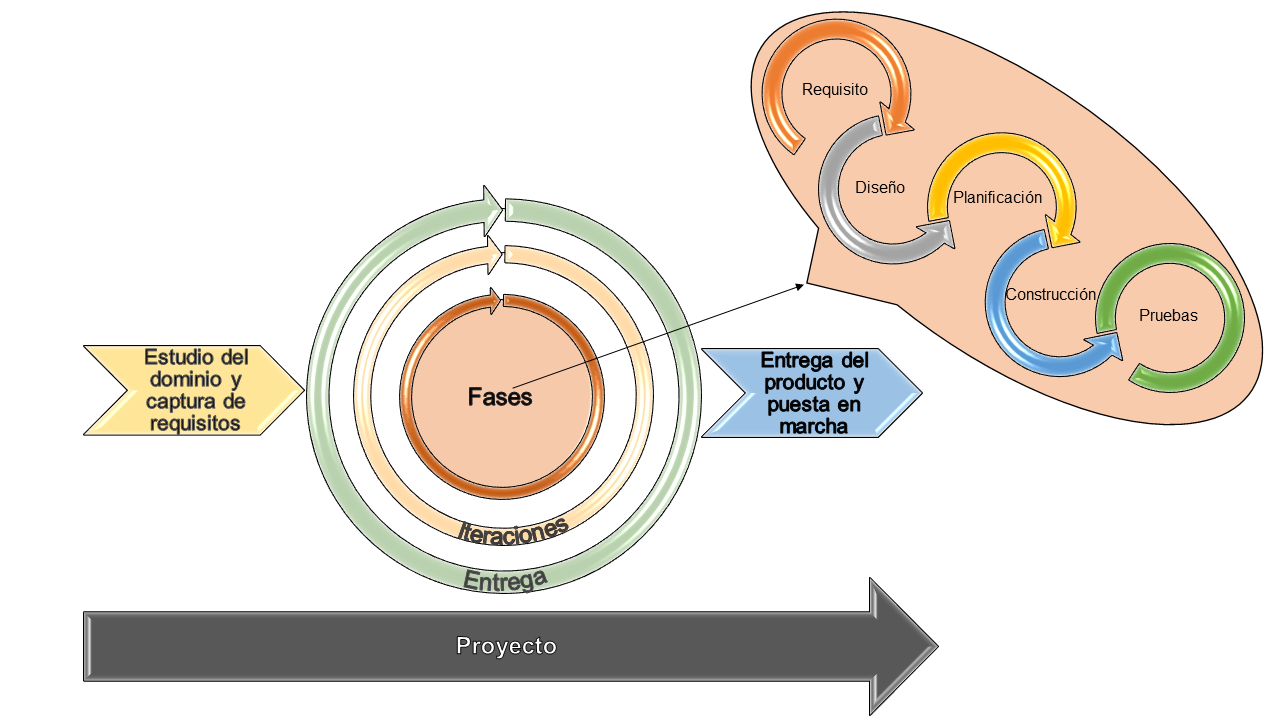
\includegraphics[width=1.1\textwidth]{Imagenes/Proceso_Proyecto.png}
    \caption{\label{fig: Proceso_Proyecto}Proceso utilizado en el proyecto}
\end{figure}